\section{Implementation}\label{sec:web_ping_impl}

To measure Internet connectivity from a users browser we had to to develop ways to collect data via a user's browser, and find ways of distributing the site to users.

\subsection{Data Collection}
JavaScript does not have an easy or well-supported method for client-side browsers to measure Internet connectivity. After researching alternatives to the network information \api, we settled on the idea of timing how long it takes for the client to load small images. Early prototypes were based on a similar tool called PingJS \cite{Frederic2016a}. To collect data, the site dynamically inserts \html \texttt{img} tags pointing to a number of small resources, each owned by one of the top 45 sites in the \us. The site records the time prior to \texttt{img} tag insertion and again upon completion of loading; this method is shown in \cref{code:web_ping_code}. Once resources from all 45 sites have been loaded, the client packages the data into a \json object and sends it via web socket to the server, which stores the data in a MongoDB database \cite{MongoDB2019a}. 

\begin{code}[htb]
    \centering
    \small
    \begin{minted}[linenos]{js}
function ping(url) {
  return new Promise(function (resolve, reject) {
    const start = (new Date()).getTime();
    const response = function () {
      let delta = ((new Date()).getTime() - start);
      resolve(delta);
    };
    request_image(url).then(response).catch(reason => reject(reason));
  });
}
    \end{minted}
    \caption{JavaScript "ping" function}
    \label{code:web_ping_code}
\end{code}


\subsection{Selection of Loaded Resources}
Initially we decided to load favicons as our images. Favicons are small images that browsers use to display an icon for the site, usually in the address bar. These images work well because they were easy to find and every website had them. Unfortunately they often varied greatly in size. Ideally all of the images loaded would have been under 1500 bytes so that they would fit in a single \tcp packet. To get the consistency and small image size needed, we developed an extension for the Chrome web browser that visits each of the top 45 sites and loads all of the images available, choosing and outputting the smallest one; a complete list may be found in \cref{sec:sites_list}. Unfortunately, a few of the chosen images were in a file format that was not readable by some browsers and as a result fewer data points were received from those sites.

\subsection{Site Ping Front End}

For the website itself we used the JavaScript Library \texttt{D3.js} ("D3") to draw maps. D3 is a library specifically designed for visualization of large data sets \cite{Bostock2011a}. To draw the states themselves, D3 loads a \json file containing a definition of the map and renders it as an \svg image on the screen. To draw points for each city, collected data is passed into D3. D3 then converts the longitude and latitude to coordinates on the screen and uses a color gradient based on \rtt to determine the color of the dot. An example of such a map is displayed in \cref{fig:siteping_city}.

Initially, we used the absolute minimum and maximum values of the data to determine the limits of the gradient, but we found that color gradients would often be skewed towards outliers. To solve this problem, we switched to using the \iqr of the data set for the color gradient. All of the points outside this range are displayed as pure red or pure white. This eliminates outlier effects while staying fast enough to be performed on the server or in the browser, as opposed to slower methods like z-score filtering.

\begin{figure}[htb]
    \centering
    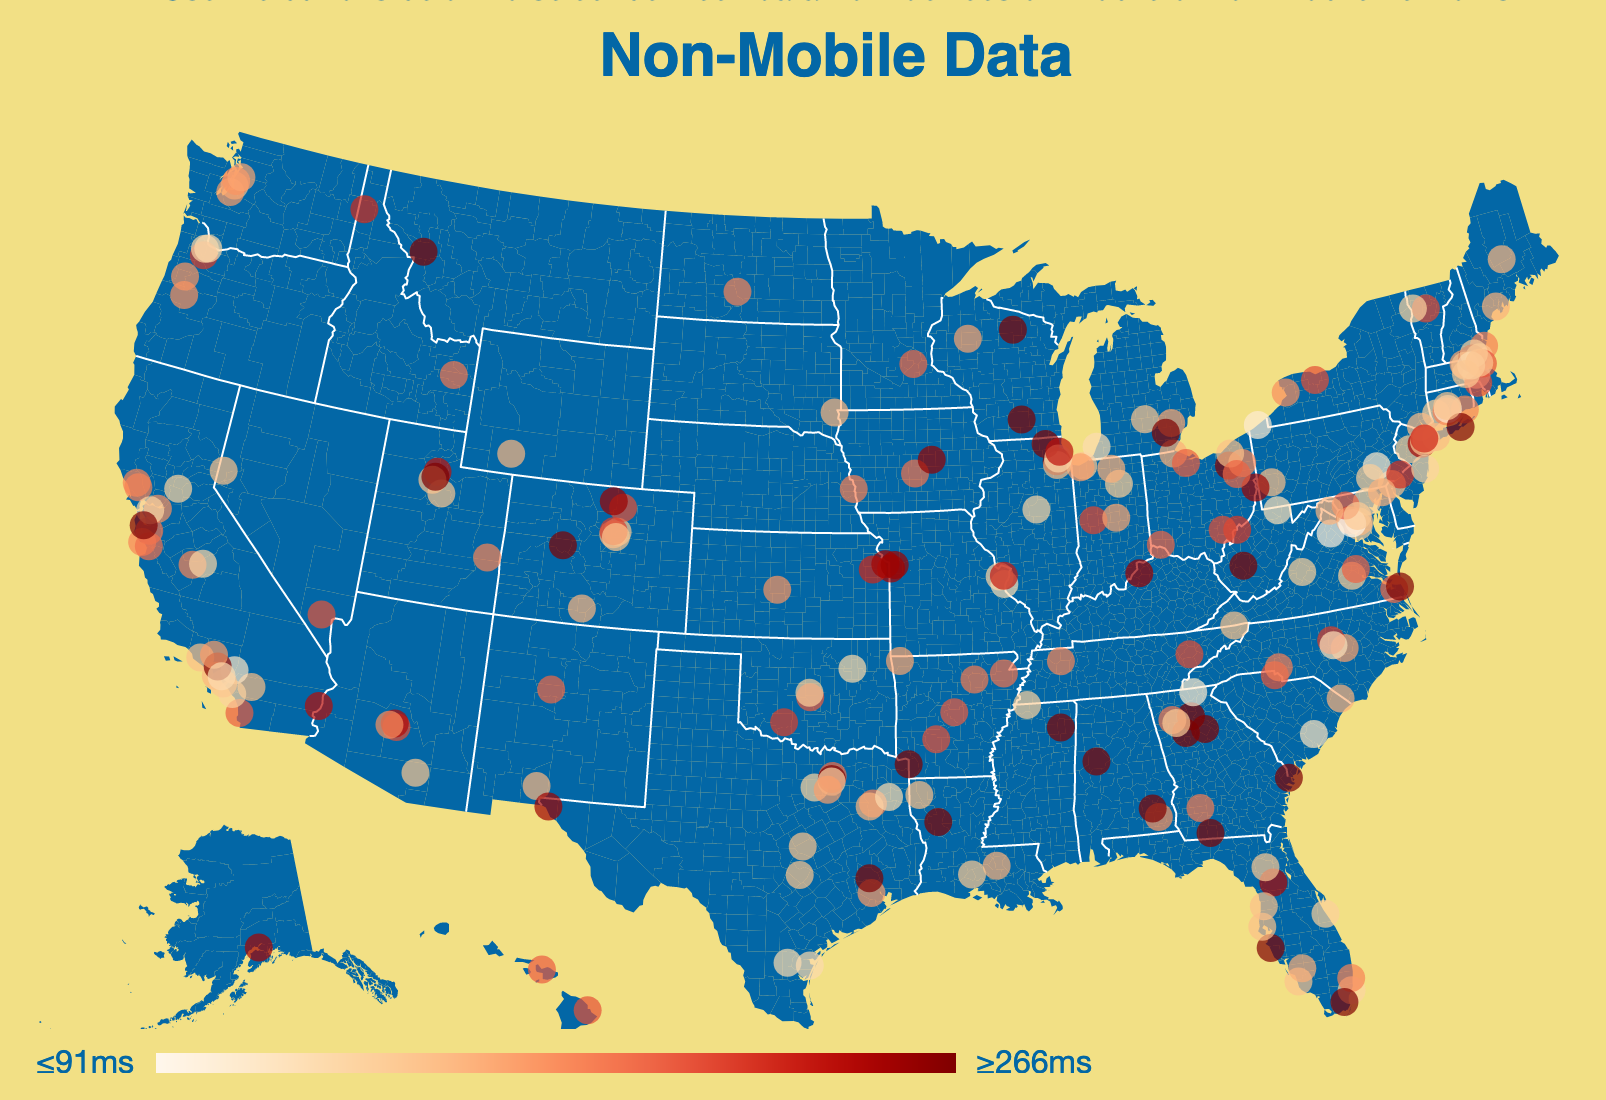
\includegraphics[width=0.75\textwidth]{siteping/cityview.png}
    \caption{Site ping city view}
    \label{fig:siteping_city}
\end{figure}

\subsection{Back End and Database}

When a client sends data to the server, the server uses  geolocation to assign the data a latitude and longitude. All of this information is stored in the database, and additionally is sent via web sockets to all of the other connected clients so the site map can update in real time. For the back-end database, we chose to use MongoDB to host all of our data \cite{MongoDB2019a}, which is queried by the server when a client connects. We chose MongoDB because of its simple and free cloud hosting platform (known as Atlas), as well as the ease of integration with NodeJS (our chosen server platform) \cite{OpenJSFoundation2019a}. The backend web server was a NodeJS server hosted on an \aws \ecc.

\subsection{Distribution}

We used multiple methods to distribute the site to people across the \us. These methods included posting to social media, using crowd sourcing, and word of mouth. To track site usage and gauge the success of these methods, we used Google Analytics, a website analytics tool. Analytics uses embedded JavaScript that gathers information about the user's browser and activity. The script can also read other cookies and metadata to determine where the user came from and how long they remained on the site. Finally, the collected information is encoded into the metadata of a request for a one pixel image \cite{Googlea}.

\subsubsection{Reddit}

The site was first properly distributed on Reddit, a popular message board and content aggregation site. We posted in two communities, \href{https://reddit.com/r/dataisbeautiful}{/r/dataisbeautiful} (14.2 million readers) and \href{https://reddit.com/r/samplesize}{/r/samplesize} (121k readers). Unfortunately, posting on Reddit proved unsuccessful and gained only around 10 views. Our posts failed to gain traction on either of these subreddits and thus few people saw them.

\subsubsection{Facebook}

One of our most successful methods for distributing the site was through Facebook. Initially, one of our members posted it on his own personal page, after which the site received a few views. Soon afterwards, a family member posted the link into the \wpi parents' Facebook group, resulting 125 views across the \us. Finally, a group member posted the link to four of the \wpi undergraduate Facebook groups, resulting in a further 70 views of the site. We intentionally waited to post to the \wpi undergraduates Facebook group until winter break started, hoping to maximize geographic diversity. The timeline of visits to the site originating from Facebook is displayed in \cref{fig:siteping_facebook_usage}. Despite this distribution, geographic diversity was limited to areas where family lives or \wpi undergraduates are typically from -- Colorado and the Northeast, respectively.

\begin{figure}[tb]
    \centering
    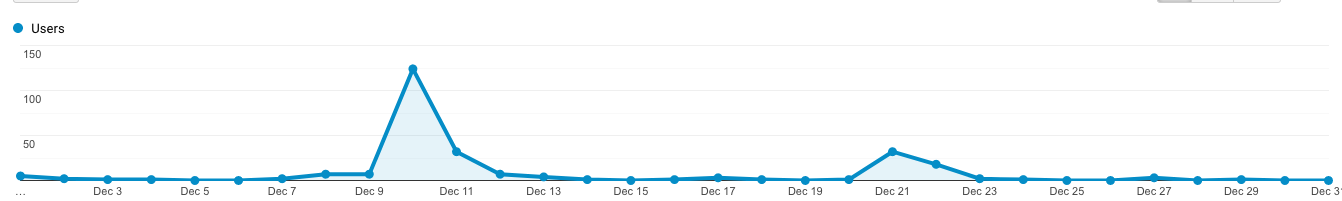
\includegraphics{siteping/usage/facebook-usage.png}
    \caption{Facebook site visits over time}
    \label{fig:siteping_facebook_usage}
\end{figure}

\subsubsection{Amazon Mechanical Turk}

To reach people in states lacking data, we turned to Amazon's Mechanical Turk service. Mechanical Turk is a crowd sourcing platform that allows people to pay others ("workers") to complete small online tasks ("HITs"\footnote{Human Intelligence Tasks}). We paid 1-50 cents for users in states that we had little data for, with higher incentives for states with sparser results. When someone selected our task, they were directed to a special \url on the site ping website. After they began data collection and waited for two cycles worth of data, they were given a token which they copied and pasted into Mechanical Turk to ensure that they actually completed the task. The tokens were generated using a \jwt module for NodeJS. Once the worker submitted the task, an \aws Lambda (with the same server-side secret used to generate the token), validated the token and approved payment. Using Mechanical Turk resulted in an additional 221 visits to the site, bringing the total of covered states up to 47. \Cref{fig:siteping_mturk_distribution} shows the nationwide distribution of Mechanical Turk users. Note that this includes users that visited the site but did not complete the task (including completing it incorrectly and returning it).

\begin{figure}[ht]
% \begin{wrapfigure}[12]{R}{0.55\textwidth}
    \centering
    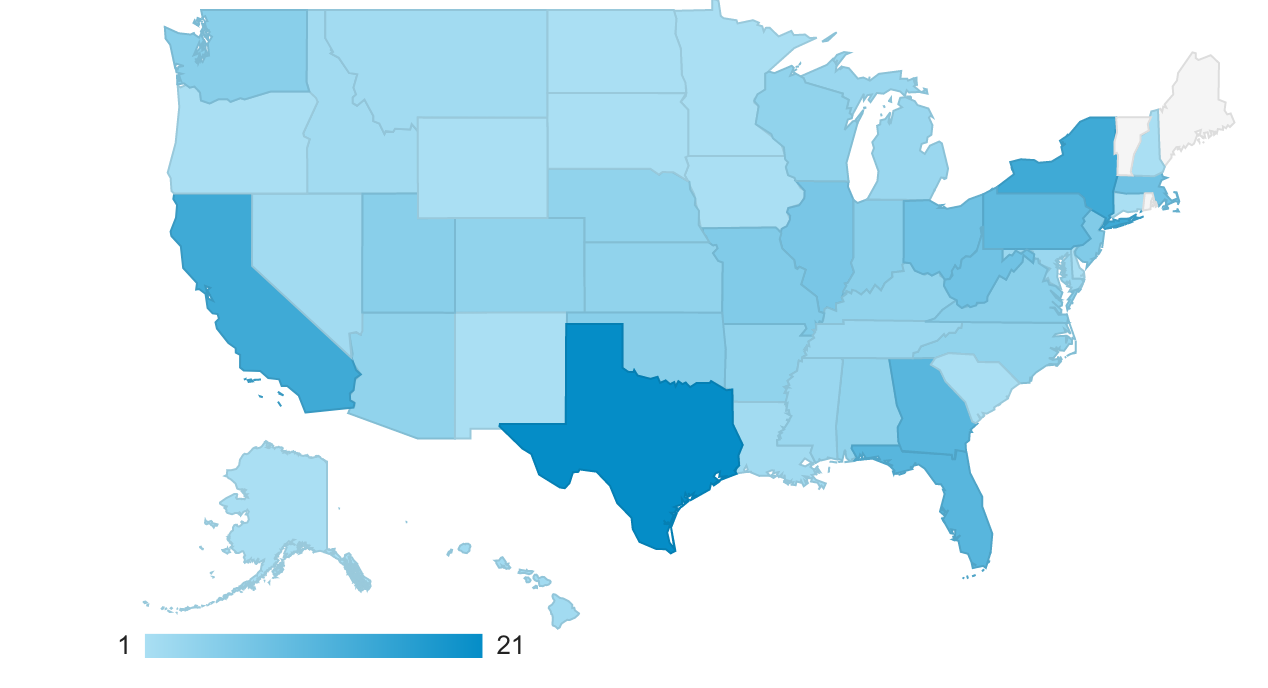
\includegraphics[width=0.55\textwidth]{siteping/usage/mturk-distribution.png}
    \caption{Involvement from Mechanical Turk by state}
    \label{fig:siteping_mturk_distribution}
% \end{wrapfigure}
\end{figure}

